\vspace{-0.2cm}
\section{Background}\label{ch4:sec:Background}
This section offers an overview of the concepts and technologies employed in this paper.
% \vspace{-3cm}
\subsection{Offline Reinforcement Learning}
% Unlike the supervised machine learning algorithm, RL algorithm do not depend on the true value for training. An RL agent, during the training phase, constantly interacts with the system to evaluate the policy generated by the policy neural network or otherwise the actor network and train itself using the reward returned by the environment or the system. This method is hence called online RL and is not suitable for real-world settings such as autonomous driving, robot control, plat operations etc. where random actions cannot be applied to the system on account of plant security or cost involved. Therefore the offline RL aims to use the prior collected data from experimentation or random human demonstrations to learn the behavior and thereby reduce/ remove the interactions with the system. 

% Unlike supervised machine learning algorithms, RL algorithms do not depend on labeled data for training. Instead, an RL agent interacts with the system, evaluates the policy by testing the actions directly on the system, and trains by using the reward returned by the environment. 
% % Akhilesh, I moved the generic RL description and maths first. Then we dive into limitations of online RL
% % Andy: Sounds good
% RL is represented by using a Markov decision process, $\mathcal{M} := (\mathcal{S},\mathcal{A}, \mathcal{R}, \mathbf{T}, \gamma)$, where $\mathcal{S}$ is the set of states that are observable information of the environment; $\mathcal{A}$ is the action space; $\mathcal{R}$ is the reward function, which is a mapping from $(\mathcal{S} \times \mathcal{A} \times \mathcal{S}) \rightarrow \mathbb{R}$; $\mathbf{T}$ is the transition probability function, $\mathcal{S} \times \mathcal{A} \rightarrow \mathcal{S}$, following which the transition from the present state $s(t)$ to the next state $s(t+1)$ occurs under the action $a(t)$ while obtaining the reward $r(s,a)$; and $\gamma \in [0,1]$ is the discount factor, which determines how much importance the agent has to give to the long-term rewards rather than the immediate rewards.   The goal of any RL agent is to find a policy $\pi$, which is a mapping from each state in $\mathcal{S}$ to $\mathcal{A}$, that maximizes the total sum of discounted rewards (called the return or the $Q$ value) along the trajectory of experience. 

% This online RL approach can be unsuitable, however, for certain real-world applications such as autonomous driving or robot control, where random actions cannot be applied to a live system because of safety or cost concerns. In the HPC domain, training an RL agent online can induce both computational and communication overhead due to the competition between the training algorithm and run time application for resources. This makes the data corrupted and unsuitable for learning. Another possibility is to separate the training node from the application node, which introduces the challenges of latency between observation and control. Therefore, in this paper we use offline RL~\cite{levine2020offline} to learn a policy from a static, pre-collected dataset that are easily available for HPC scientists. 
% This dataset, which is considerably smaller than the full action-state domain under consideration, is gathered by using arbitrary policies. The offline training
Reinforcement learning (RL) formulates control as a sequential decision-making problem, typically modeled as a Markov decision process (MDP) $\mathcal{M} := (\mathcal{S}, \mathcal{A}, \mathcal{R}, \mathbf{T}, \gamma)$, where an agent observes the system state $s \in \mathcal{S}$, selects an action $a \in \mathcal{A}$, and receives a reward $r \in \mathcal{R}$. The objective is to learn a policy $\pi : \mathcal{S} \rightarrow \mathcal{A}$ that maximizes the expected discounted return.
% The algorithm then uses this dataset to learn an optimal policy without further system interactions. We note that no mainstream RL algorithm, including Conservative Q-learning (CQL) \cite{levine2020offline}, is capable of taking actions it has never seen during training. Therefore, we ensure that the dataset exhaustively samples the action space at least once across different applications and hardware combinations. 

\iffalse 
% Akhilesh, we have already said that online RL is not acceptable for us. Let us skip this to save space
While RL is commonly trained through online interaction with the environment, such an approach is often impractical in real-world systems. In HPC settings, online training can interfere with application execution, introduce measurement noise, and incur unacceptable computational overhead. To avoid these issues, we adopt offline RL~\cite{levine2020offline}, which learns control policies from static, pre-collected datasets without requiring interaction with the live system during training.
\fi 

% Akhilesh, I think one of the concerns was that this dataset was too small.
% Andy: Yes due to which we have a smaller network and I am putting that information in the experiments.
% OK
% In an offline RL setting such as the Q-learning we use in this paper, we cannot evaluate an unaccounted state-action pair during the training phase. Instead, we rely on the ability of the Q-network to learn from the available dataset a value function, given any state. A common challenge associated with using such an offline dataset for training an RL agent is distributional shift. This refers to a situation where the distribution of states and actions being encountered during training differs from the real-world behavior, thereby adversely impacting the trained agent performance. Another challenge associated with offline RL is its suboptimal performance when trained using a random policy.
% Here we use CQL \cite{levine2020offline} for training the RL-agent, a version of offline RL that regularizes the policy to avoid overestimation of the Q-values. By carefully choosing the learning parameters, we train an offline CQL agent from a previously collected dataset without overfitting. However, the knowledge of the system to be controlled can help populate the dataset with greedy policies to ensure near optimal behavior of the controller.
% We recall here the mathematical form of the loss function of CQL below for the reader’s understanding.

In an offline RL setting such as the Q-learning approach used in this paper, unobserved state–action pairs cannot be evaluated during training. Instead, learning relies on the ability of the Q-network to approximate a value function from the available dataset. A common challenge in this setting is distributional shift, which arises when the distribution of states and actions encountered during training differs from that observed at deployment, potentially degrading performance. Another limitation of offline RL is suboptimal learning when trained solely from random policies.

To address these challenges, we employ Conservative Q-Learning (CQL)~\cite{levine2020offline}, which regularizes Q-value estimation to mitigate overestimation under distributional shift. By carefully selecting learning parameters, we train an offline CQL agent from a previously collected dataset without overfitting. Moreover, incorporating domain knowledge of the controlled system enables the dataset to be populated with informative (greedy) behaviors, improving the quality of the learned policy. 

% Akhilesh, the following though nice probably is not needed to understand anything that comes next
% So, to save space, I am commenting it out
\iffalse 
We recall the mathematical form of the CQL loss function below for completeness.


%\vspace{-0.5cm}
% \begin{equation}
% \begin{aligned}
%     \min_Q \overbrace{\max_{\mu} \Big(\mathbb{E}_{s\sim \mathcal{D}}\mathbb{E}_{a(t) \sim \mu(a(t) \vert s(t))}[Q(s(t),a(t))]} ^{\text{Minimize the big Q-values}}- \overbrace{\mathbb{E}_{s(t),a(t) \sim \mathcal{D}}[Q(s(t),a(t))]\Big)}^{\text{Maximize the data Q-values}} \\ + \underbrace{\frac{1}{2\alpha}\mathbb{E}_{s(t),a(t),s(t+1) \sim \mathcal{D}}[(Q(s(t),a(t))-r(s(t),a(t)) - \gamma \mathbb{E}_{a(t+1) \sim \pi_{\theta}(a(t+1)\vert s(t+1))[Q(s(t+1),a(t+1))]})^2]}_{\text{Standard TD error}} 
% \end{aligned}
% \label{eq:CQL}
% \end{equation}
% \vspace{-0.4cm}
\begin{equation}
% \vspace{-0.2cm}
\small
\begin{aligned}
    \min_Q \ & \overbrace{\max_{\mu} \Big(\mathbb{E}_{s\sim \mathcal{D}}\mathbb{E}_{a_t \sim \mu(a_t \vert s_t)}[Q(s_t,a_t)] - \mathbb{E}_{s_t,a_t \sim \mathcal{D}}[Q(s_t,a_t)]\Big)}^{\text{Conservative term}} \\
    & + \frac{1}{2\alpha}\mathbb{E}_{s_t,a_t,s_{t+1} \sim \mathcal{D}}[(Q(s_t,a_t) - r(s_t,a_t) \\& - \gamma \mathbb{E}_{a_{t+1} \sim \pi_{\theta}(a_{t+1} \vert s_{t+1})}[Q(s_{t+1},a_{t+1})])^2],
\end{aligned}
\label{eq:CQL}
% \vspace{-0.1cm}
\end{equation}
where $s_t,a_t$ represent, respectively, the present state and  action, $\mathbb{E}$ is the notation for expected value, $\mu$ is the current policy from which the action $a_t$ is chosen (initialized as random policy), $\mathcal{D}$ is the state distribution under policy $\mu$, $\alpha$ is the conservative learning factor that determines how the RL agent reacts to out of distribution data, and $\pi_{\theta}$ represents the parameterized target policy, where $\theta$ represents the weights of the Q-network.
\fi 
% In Equation~\ref{eq:CQL}, the first part (regularization) minimizes distributional shift while second part minimizes the Bellman error.
 
% \subsection{Reward Function}
% Initially, we used a straightforward reward function that simply inverts the power consumption within each scheduling window: $R1(s, a) = -power$, where $s$ represents the progress value and $a$ the PCAP taken. While this function favors configurations with lower power usage, it does not account for performance impacts.

% To more effectively balance energy conservation with performance, we examine a metric that measures the performance divided by power. This can be seen as a variation of the energy-delay product (EDP), where delay is interpreted as the average time per instruction. Given our focus on HPC workloads, it's important to heavily penalize increased delays, which prompts us to consider a third potential reward function: $(progress)^3/PCAP$, resembling an inverse of $(EDP)^2$ on an instruction basis. To ensure a consistent increase in rewards, we scale $(progress)^2/PCAP$ and $(progress)^3/PCAP$ by a fixed constant $c$ where $(c >= 10)$, yielding two new reward function alternatives $R2(s, a) =  \times (progress)^2/W$ and $R3(s, a) = c \times (progress)^3/W$.

% In Section 5.6, we validate empirically that our preferred reward function R3(s, a) = (c×IPC)^3/W, drives the strongest overall performance, making it the chosen reward function for our system.
% \begin{algorithm}
%     \SetAlgoLined
%     \KwIn{Finite Dataset $\mathcal{D}$, Learning Rate $\alpha$, Discount factor $\gamma$}
%     \KwData{Critic Net $Q_\phi$}
%     \KwIn{Replay Buffer of size $b$ with transitions and rewards $\mathcal{B} \leftarrow \{(s_i, a_i, r_i, s_i')\}$}
%     \For{$\text{training iteration } t \in \{0, \dots, T\}$}{
%         \For{$i \leftarrow 0$ \KwTo $b$}{
%             Sample $(s_i, a_i, r_i, s_i')$ uniformly from $\mathcal{D}$\;
%         }
%         % $\tilde{s}_j \leftarrow g_\psi(s_j)$\;
%         $L_{\text{critic}} \leftarrow \frac{1}{B} \sum_{i=0}^{B} \left( Q_\phi({s}_i', a_i) - \mathbb{E}_{a' \sim \pi_\theta({s}_i')} \left[ (r_i + \nabla\gamma(Q_\phi({s}_i, a')))^2 \right] \right)$\;
%         % $\hat{A}(\tilde{s}_i, a_i) \leftarrow Q_\phi(\tilde{s}_i, a_i) - \frac{1}{k} \sum_{j=0}^{k} Q_\phi(\tilde{s}_i, a_j' \sim \pi_\theta(\tilde{s}_i))$\;
%         % $L_{\text{actor}} \leftarrow \frac{1}{B} \sum_{i=0}^{B} \left( -1_{\{ \hat{A}(\tilde{s}_i, a_i) > 0 \}} \log \pi_\theta(a_i | \tilde{s}_i) \right)$\;
%         % $\psi \leftarrow \psi - \alpha \nabla_\psi L_{\text{critic}}$\;
%         $\phi \leftarrow \phi - \alpha \nabla_\phi L_{\text{critic}}$\;
%         % $\theta \leftarrow \theta - \alpha \nabla_\theta L_{\text{actor}}$\;
%     }
%     \KwOut{Trained Scheduling Policy $argmax(Q_\phi(s))$}
%     \caption{Offline Training Algorithm}
% \end{algorithm}

% \begin{figure*}[htb]
%     \centering
%     \begin{subfigure}[b]{0.5\textwidth}
%         \centering
%         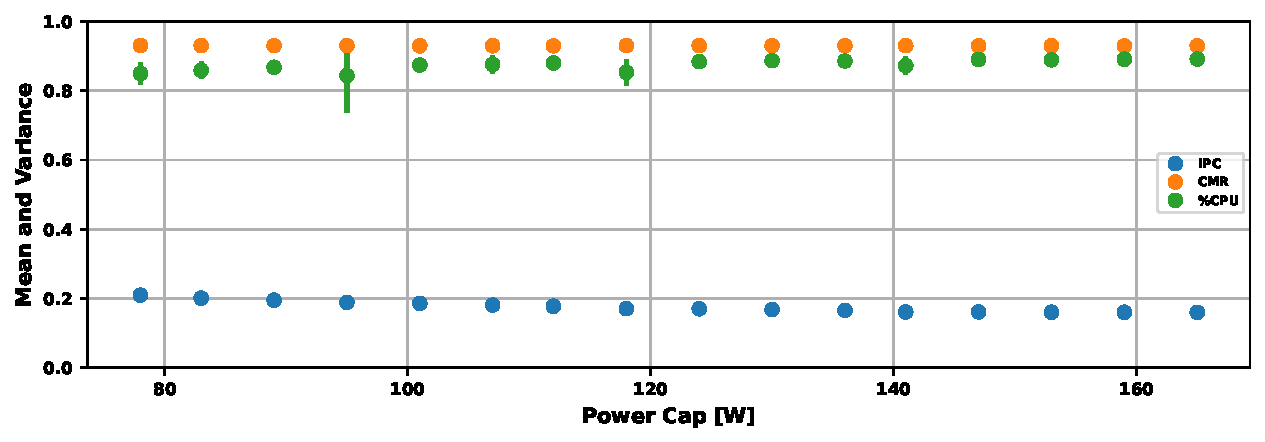
\includegraphics[width=\textwidth]{Figures/PAPI_stats_ones-stream-full.pdf}
%         % \caption{$Stream-Full$}
%         \label{fig:stream_perf}
%     \end{subfigure}\hfill
%     \begin{subfigure}[b]{0.5\textwidth}
%         \centering
%         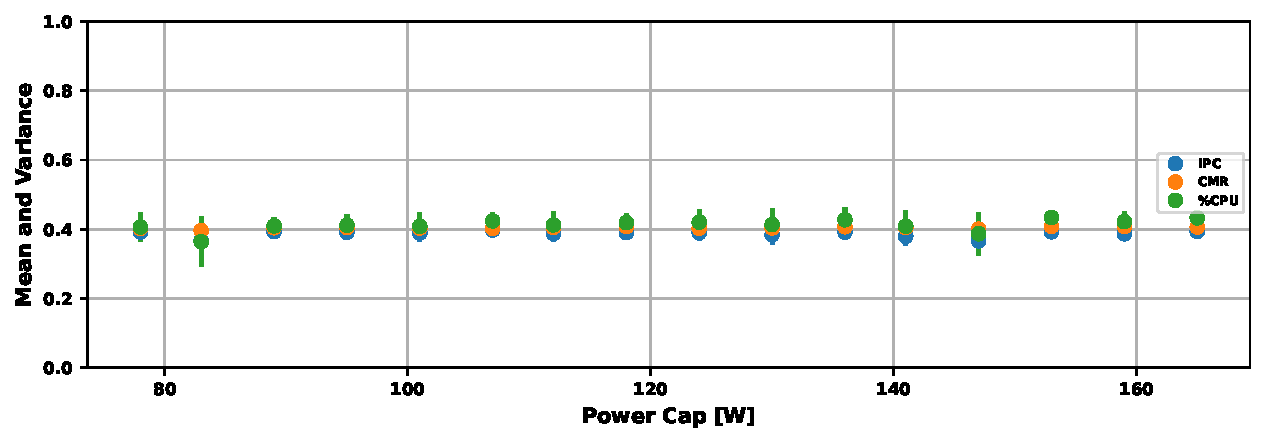
\includegraphics[width=\textwidth]{Figures/PAPI_stats_ones-npb-ep.pdf}
%         % \caption{$NPB-EP$}
%         \label{fig:ep_perf}
%     \end{subfigure}
%     \vspace{-1cm}
%     \caption{Average ($\mu$) and Standard deviation ($\sigma$) of IPC, CPU and CMR at various power levels for two of our benchmarks (Stream-full and NPB-EP). The experiments were repeated 10 times for each of the power caps.}
%     \label{fig:mu_sigma}
% %    \Description{Motivating example}
% \end{figure*}

% \begin{figure*}[htb]
%     \centering
%     \begin{subfigure}[b]{0.5\textwidth}
%         \centering
%         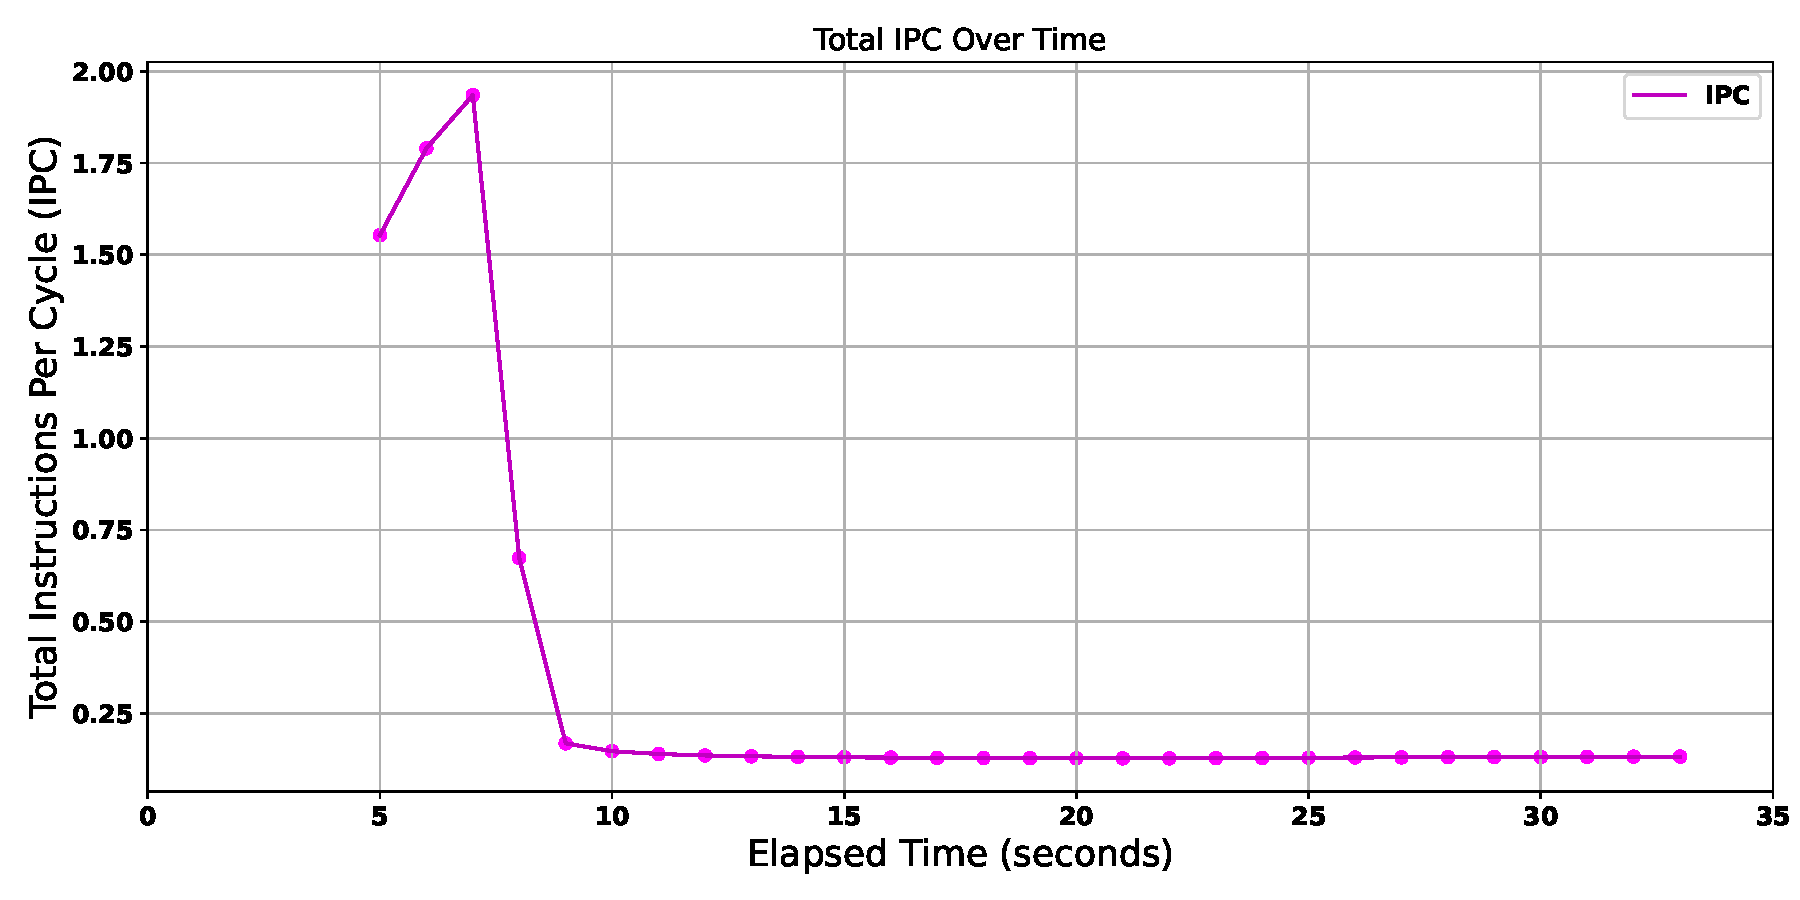
\includegraphics[width=\textwidth]{Figures/IPC_plot.pdf}
%         \caption{$IPC$}
%         \label{fig:IPC}
%     \end{subfigure}\hfill
%     \begin{subfigure}[b]{0.5\textwidth}
%         \centering
%         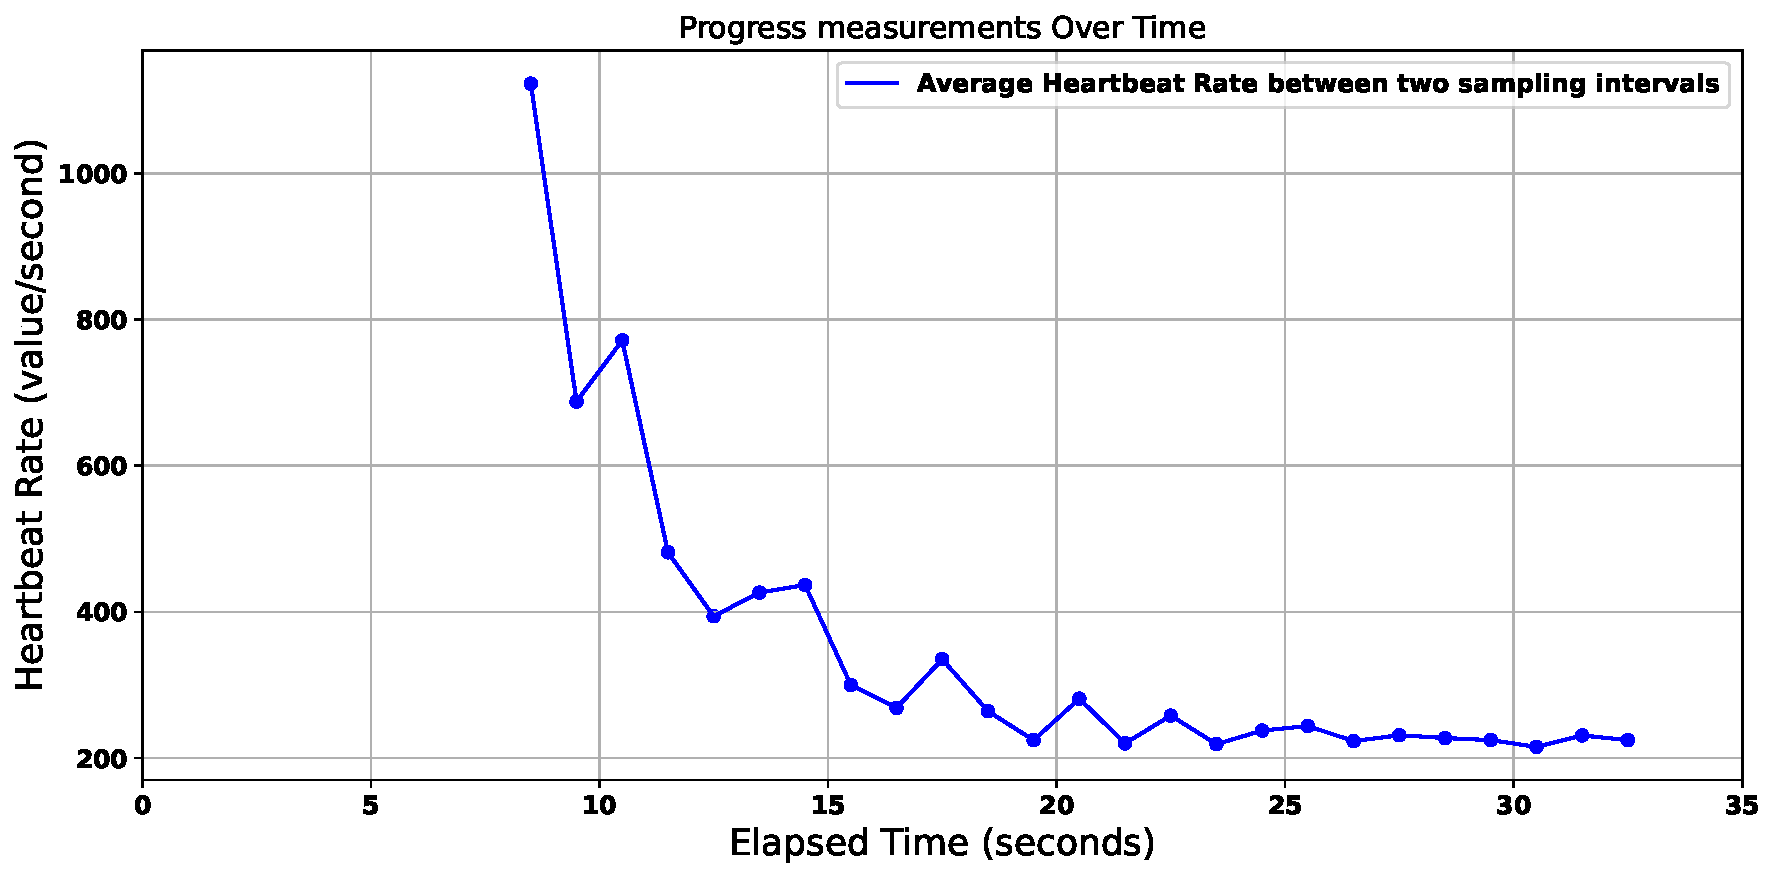
\includegraphics[width=\textwidth]{Figures/progress.pdf}
%         \caption{$Progress$}
%         \label{fig:progress}
%     \end{subfigure}
%     \caption{Comparison of $IPC$ and $progress$ during the runtime of an application (XS-Bench) with progress values displaying more performance granularity.}
%     \label{fig:perf_granularity}
%     \Description{Motivating example}
% \end{figure*}
% \vspace{-0.1cm}

\subsection{Measuring Application Performance through Hardware Performance Counters} \label{ch4:bg:subsec:Applications_vs_perf}

% Akhilesh, I added this sentence otherwise there was no justification why  we are doing this
Training the offline models as suggested above requires a dataset of application performance
on different hardware. However, 
different applications can illustrate differing performance on a given hardware architecture.
This performance is influenced by hardware characteristics such
as memory bandwidth, CPU cores, and cache size. To capture this complex
application-hardware interaction in the dataset, we leverage a set of hardware performance
counters while running applications on the target system. Specifically, we rely on the
Performance Application Programming Interface (PAPI)~\cite{mucci1999papi} to provide portable access to hardware performance counters.  PAPI offers easy access to a variety of counters through direct queries on the hardware model-specific registers. These measurements are representative of hardware-specific and application-specific data movement, or a combination of both.

To optimize energy efficiency while preserving performance, we focus on a small set of key performance metrics: total instructions issued ($TOT\_INS$), total clock cycles ($TOT\_CYC$), total last-level cache accesses ($L3\_TCA$), last-level cache misses ($L3\_TCM$), and cycles stalled because of resource contention ($RES\_STL$). We chose these key metrics for two reasons. First, these readings are available instantaneously and simultaneously during every sampling interval. Second, they are direct and sufficient indicators of the rate of data flow within and between the CPU cores and memory. Furthermore, because direct usage of these metrics would call for a large trained network and necessitate additional data processing, we follow insights from other research~\cite{wittmann2016chip,rane2014enhancing} in computing a set of \textit{derived metrics} (instructions per cycle ($IPC$), the ratio of stalled cycles to total cycles (often equated with CPU utilization, noted as $STL$), and last-level cache miss rate ($CMR$)) which facilitate a more detailed analysis of runtime behavior.  

\textbf{Key Insight:} Based on findings from previous works, we note that these metrics should not be viewed in isolation as definitive indicators of performance, since varying IPC values, for example, can still lead to the same execution time. Nonetheless, these derived metrics serve as valuable proxies to discern application characteristics, including its arithmetic intensity or whether the application is memory-bounded and thus can operate efficiently within a lower power budget.

% Figure \ref{fig:res_stl_cycle} gives the derived metric total cycles stalled divided by total number of cycles between two sampling instants for different applications for varying power levels. This figure shows how the characteristic value differs on the same hardware for different applications for varying power caps.
% \begin{figure}
%     \centering
%     \includegraphics[width=\linewidth]{Figures/derived_cyc.pdf}
%     \caption{$\frac{\text{total stalled cycles}}{\text{total cycles}}$ for different benchmark applications. %The stream applications are all memory bound while the ep application is compute bound}
%     \Description{The relationship between percentage CPU usage with varying input power.}
%     \label{fig:res_stl_cycle}
% \end{figure}


% Figure \ref{fig:mu_sigma} depicts the mean ($\mu$) and variance ($\sigma$) of these values over an execution under a constant power cap. of each of these metrics with varying power caps across the node for two different applications. The experiments were performed on an Intel processor and repeated 10 times to get the statistics. Figure shows a non linear relationship that exists between the memory access variables and the power cap of the node for different applications and these characteristics together acts as a fingerprint of the application. 
% \textcolor{red}{comment on the similarity of the plots between the ones-stream-full, copy and triad}



% \begin{figure}
%     \centering
%     \includegraphics[width=\linewidth]{Figures/derived_One_stat_vs_Power.pdf}
%     \caption{Correlation of the application with the derived metrics from the PAPI measurements showing mean and variance over 10 independent runs.}
%     \label{fig:mu_sigma}
%     \Description{The relationship between other PAPI measurements usage with varying input power.}
% \end{figure}

%\subsection{Application-aware Performance Measurement} \label{ch4:bg:subsec:Performance_Measurement}
\subsection{Capturing Application Progress in the Dataset} \label{ch4:bg:subsec:Performance_Measurement}
% Akhilesh, our work is application-agnostic. But the above heading will raise eyebrows. How do we reconcile this contradiction? IN other words, how can we claim that by doing application-aware measurements we can do application-agnostic power optimization?
% Akhilesh, I changed the heading above

We augment our monitoring of application behavior by adding a notion of \textit{progress}, or \textit{heartbeats}, to our system. This measure is obtained by a lightweight instrumentation of the applications under study.  Our approach follows the work of Ramesh et al.~\cite{ramesh2019understanding} and follows the instrumentation steps outlined by Cerf et al.~\cite{cerf2021sustaining}.
The role of this progress measurement is to highlight the potential for an application to be busy-waiting for some resource in the system and thus be active but not making useful use of compute power.

We redefine the progress measurement equation introduced in~\cite{ramesh2019understanding} by considering the number of heartbeats received between two sampling (control) instants. The progress at time instant $t_i$ is given by Equation~\eqref{eq:progress-calculation}:
% Akhilesh, what is the relationship of i and k in the following? it is confusing. Presumably the interval i-1 to i is larger or equal to the k-1 to k, right? i.e., k-1 to k is a subwindow of the i-1 to i window (could be exactly the same)? What does all this mean i.e., semantics? why is this important?
%\vspace{-0.4cm}
%Andy: tk is the arrival time of the heartbeats between two sampling intervals (control instances). This means we are are using the value returned by our instrumentation in iterative applications as a measure of our instantaneous performance or progress. It is a proxy. I think we have added all these information in the paragraph. Let me know if it is still confusing.
% Yes, the info is there but the relevance of "i" is not mentioned and how is k related to i. But anyway there is no space to add any more explanation.
\begin{equation}
\begin{aligned}
progress(t_i) = \underset{\forall k,t_k \in [t_{i-1},t_i]}{\text{median}}\bigg(\frac{N}{t_k-t_{k-1}} \bigg),
\end{aligned}
\label{ch4:bg:eq:progress-calculation}
\end{equation}
where $N$ represents the number of heartbeats received between the time instants
$t_k$ and $t_{k-1}$. This measure of
progress can be understood as a proxy for monitoring the figure of merit
of an application at runtime. Equation \eqref{eq:progress-calculation} enables us to accurately measure progress while considering the time interval and the number of heartbeats received. It also allows us to limit the heartbeat-rate of instrumentation to avoid overflowing our infrastructure with messages, since  it is sufficient to accumulate a 
heartbeat counter on the application side and to only periodically send this
counter to our data collection and control infrastructure. 

%%\subsection{Benchmarks}
%%
%%In this paper we use a collection of well-established benchmarks to represent the behaviors of various applications and their response to power capping. The benchmarks
%%listed here are used both for training our control agent and its validation, with some of them being kept out of our training dataset and only used for validation. By using these well-established benchmarks, we hope to train our model to recognize and predict optimal power management strategies that will be applicable to a wide range of application behaviors.
%%
%%
%%% Akhilesh, in the context of this above para, what is the t_k-1 to t_k window? and what is i-1 to i from the above equation? 
%%% Andy i and i-1 is the choice of our controller. The RL controller. In our case it is decided by the time when all the sensor information is available. Nearly 2s. k and k-1 corresponds to the time between completion of one outer loop.
%%
%%% moved here so it appears in the right place
%%\begin{table*}[htb]
%%    \centering
%%    \caption{Detailed description of our benchmarks, including their type, parameters, and average performance metrics when running without a power cap.}
%%    \label{ch4:tab:performance_metrics}
%%    \resizebox{\linewidth}{!}{%
%%        \begin{tabular}{|c|c|c|c|c|c|c|c|c|c|}
%%            \hline
%%            \textbf{Benchmark} & \textbf{Prob Size} & \textbf{Iter.} & \textbf{Avg. IPC} & \textbf{Avg. CMR} & \textbf{Avg. STL} & \textbf{Avg. Prog.} \textbf{[\unit{Hz}]} & \textbf{Avg. ET}\textbf{[\unit{s}]} & \textbf{Avg. Energy} \textbf{[\unit{kJ}]} & \textbf{Ari. Int. (FLOPs/Byte)} \\
%%            \hline
%%            {\textbf{Stream-Scale}}  & 33554432 & 10000 & 0.20 & 0.89 & 0.84 & 285.20 & 34.40 & 5.59 & 1.62 \\
%%            \hline
%%            {\textbf{Stream-Triad}}  & 33554432 & 10000 & 0.18 & 0.94 & 0.83 & 200.03 & 50.80 & 7.93 & 1.41 \\
%%            \hline
%%            {\textbf{NPB-EP}}  & Class-W & 1000 & 0.57 & 0.13 & 0.48 & 13.61 & 73.80 & 10.33 & 53.99 \\
%%            \hline
%%            {\textbf{NPB-IS}}  & Class-B & 1000 & 0.50 & 0.86 & 0.68 & 8.44 & 117.33 & 18.99 & 1.21 \\
%%            \hline
%%            \hline
%%            {\textbf{Stream-Add}}  & 33554432 & 10000 & 0.15 & 0.94 & 0.85 & 201.06 & 50.40 & 7.84 & 1.36 \\
%%            \hline
%%            {\textbf{Stream-Copy}}    & 33554432 & 10000 & 0.17 & 0.89 & 0.84 & 282.43 & 35.50 & 5.66 & 1.63 \\
%%            \hline
%%            {\textbf{Stream-Full}}  & 33554432 & 10000 & 0.16 & 0.93 & 0.70 & 49.31 & 222.40 & 34.99 & 1.45 \\
%%            \hline
%%            {\textbf{Stream-Phase}}  & 33554432 & 10000 & 0.17 & 0.91 & 0.88 & 240.16 & 83.00 & 13.48 & 1.45 \\ 
%%            \hline
%%            {\textbf{NPB-MG}}  & Class-B & 1000 & 0.47 & 0.809 & 0.54 & 40.3 & 22.23 & 55.5 & 1.45 \\
%%            \hline
%%            {\textbf{NPB-FT}}  & Class-B & 500 & 0.82 & 0.43 & 0.296 & 13.23 & 35.10 & 45.47 & 1.53 \\
%%            \hline
%%            {\textbf{NPB-CG}}  & Class-C & 1000 & 0.49 & 0.37 & 0.62 & 9.97 & 114.00 & 14.74 & 3.61 \\
%%            \hline
%%            {\textbf{NPB-BT}}  & Class-C & 1000 & 0.97 & 0.87 & 0.30 & 6.22 & 166.00 & 23.168 & 0.54 \\
%%            \hline
%%        \end{tabular}
%%    }
%%\end{table*}
%%
%%\begin{itemize}
%%    \item \textbf{STREAM}~\cite{McCalpin1995} is a well-known benchmark designed to evaluate the memory performance and bandwidth of a system. We consider 6 versions of this benchmark, corresponding to its 4 inner kernels (add, copy, scale, and triad) with varying arithmetic intensity, as well as one version (\texttt{full}) that executes all 4 kernels as part of its outer loop. The last version, with phases, repeats the full benchmark a number of times, resulting
%%    in changes in progress rate and behavior across its execution. For all these versions, the input problem size (the size of the working arrays in memory) has a direct impact on the performance, and is chosen here so that these arrays do not fit in the last level cache on the system under study.
%%    
%%    \item \textbf{NAS} Parallel Benchmarks (NPB) consists of a collection of programs created to benchmark the performance of parallel processors using kernels that are representative of scientific applications. While there are many benchmarks in NPB, we include six here: Embarrassingly Parallel (EP) for being a representative of a compute-bound application, Integer Sort (IS) for its focus on random memory accesses, Fourier Transform (FT) for straining the cache for memory access, Multi Grid (MG) for its computational intensity, Conjugate Gradient (CG) for memory-intensive and irregular communication patterns and Block Tridiagonal (BT) for its compute intensive and irregular communication. Our implementation is inspired by the NPB-3.4-OpenMP versions. 
%%\end{itemize}
%%
%%% \begin{figure}[htb]
%%%     \centering
%%%     \begin{subfigure}[b]{0.48\textwidth}  % Adjusted width to fit side by side
%%%         \centering
%%%         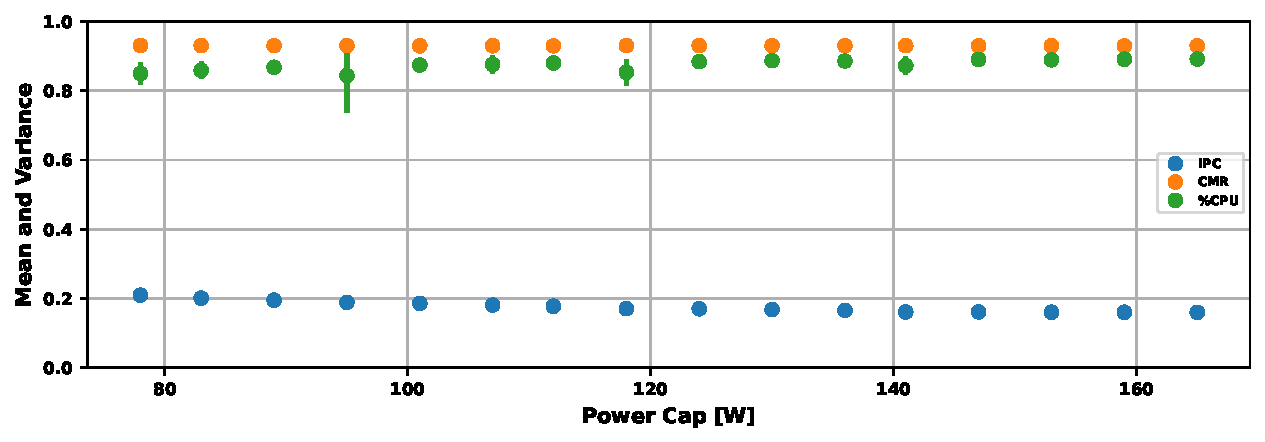
\includegraphics[width=\textwidth]{Figures/PAPI_stats_ones-stream-full.pdf}
%%%         \caption{$ONES-STREAM-FULL$}
%%%         \label{fig:stream_perf}
%%%     \end{subfigure}\hfill
%%%     \begin{subfigure}[b]{0.48\textwidth}  % Adjusted width to fit side by side
%%%         \centering
%%%         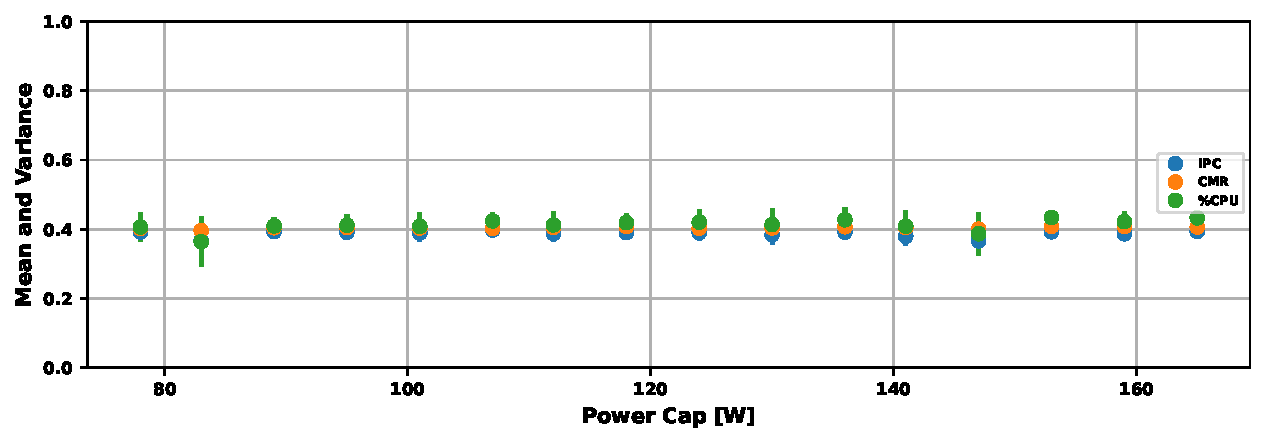
\includegraphics[width=\textwidth]{Figures/PAPI_stats_ones-npb-ep.pdf}
%%%         \caption{$ONES-NPB-EP$}
%%%         \label{fig:ep_perf}
%%%     \end{subfigure}
%%%     \caption{Average ($\mu$) and Standard deviation ($\sigma$) of IPC, CPU and CMR at various power levels for two of our benchmarks. The experiments were repeated 10 times for each of the power caps.}
%%%     \label{fig:mu_sigma}
%%%     \Description{Motivating example}
%%% \end{figure}
%%
%%
%%% To further motivate our use of both derived metrics and progress measurements, we generated plots for Instructions Per Cycle (IPC), CPU utilization, and Cache Miss Rate (CMR) across two distinct benchmark applications, each subjected to varying node power or Power Caps ($PCAP$s). These experiments were conducted on an Intel processor with $PCAP$s held constant during each application run. For each run, we computed the mean ($\mu$) and standard deviation ($\sigma$) of the derived metrics and charted them against their respective $PCAP$ values.
%%% The correlation is depicted in Figure \ref{fig:mu_sigma}. 
%%% To ensure consistency, we replicated the experiments 10 times for each application, keeping the problem size constant. The normalized results, illustrated in Figure \ref{fig:mu_sigma}, demonstrate unique differences in the metrics for memory-bound and compute-bound applications respectively.
%%% The $IPC$, $STL$, and $CMR$ values collectively constitute a distinctive vector, serving as a "fingerprint" of the application given the specific $PCAP$. Notably, the relation of performance counter metrics to $PCAP$ differs from the application's "progress" as seen in Figure \ref{fig:motivation_fig}.
%%% This observation underscores the insights of Ramesh et al. \cite{ramesh2019understanding}, highlighting the significance of measuring application progress towards achieving scientific objectives.
%%We modified these benchmarks to become iterative in nature, so that application progress is more easily identifiable: when not already a part of the benchmark, an outer loop is introduced, repeating their kernels a configurable amount of time. Each outer loop also contains our instrumentation for heartbeats, resulting in each  benchmark reporting one heartbeat per iteration. Note, the progress rate of each benchmark is different and depends on the runtime of its kernel.
%%% Table \ref{ch4:tab:performance_metrics} shows the names and associated characteristics of the applications we consider in this paper for a quick reference. 
